\aufgabe{}{

You received a dataset with 9 observations and two features:

\begin{table}[ht]
\centering
\begin{tabular}{rrrrrrrrrr|r}
\hline
& 1 & 2 & 3 & 4 & 5 & 6 & 7 & 8 & 9 & $\sum_{i = 1}^n$ \\ 
\hline
y & -7.79 & -5.37 & -4.08 & -1.97 & 0.02 & 2.05 & 1.93 & 2.16 & 2.13 & -10.92\\ 
x1 & -1.00 & -0.75 & -0.50 & -0.25 & 0.00 & 0.25 & 0.50 & 0.75 & 1.00 & 0 \\ 
x2 & 0.95 & 0.57 & 0.29 & -0.03 & 0.02 & 0.08 & 0.23 & 0.54 & 0.98 & 3.63 \\
\hline
\end{tabular}
\end{table}

The last column corresponds to the sum of values of each row.

\begin{enumerate}[a)]
\item Compute the Pearson correlation of $x_1$ and $x_2$.  
The formula is: 
$$ 
\rho(x_1, x_2) = \frac{\sum_{i = 1}^n (x_1^{(i)} - \overline{x}_1)(x_2^{(i)} - \overline{x}_2)}{\sqrt{\sum_{i = 1}^n (x_1^{(i)} - \overline{x}_1)^2} \sqrt{\sum_{i = 1}^n (x_2^{(i)} - \overline{x}_2)^2}}
$$ 
To speed up things, the individual differences to the means ($x_1^{(i)} - \overline{x_1}$, $x_2^{(i)} - \overline{x_2}$),  are given in the following table.  

\begin{table}[H]
\centering
\begin{tabular}{rrrrrrrrrr}
\hline
& 1 & 2 & 3 & 4 & 5 & 6 & 7 & 8 & 9 \\ 
\hline
$x_1^{(i)} - \overline{x_1}$ & -1.00 & -0.75 & -0.50 & -0.25 & 0.00 & 0.25 & 0.50 & 0.75 & 1.00 \\ 
$x_2^{(i)} - \overline{x_2}$ & 0.55 & 0.17 & -0.11 & -0.43 & -0.38 & -0.32 & -0.17 & 0.14 & 0.58 \\ 
\hline
\end{tabular}
\end{table}

Interprete the results. Based on $\rho(x_1, x_2)$, are $x_1$ and $x_2$ correlated? 

\vspace*{2cm}

\item Add points ($x_1$, $x_2$) to the following figure: 

\begin{center}
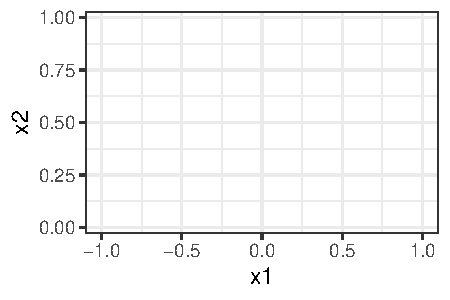
\includegraphics[width=\maxwidth]{figure/add_Points_x1_x2.pdf}
\end{center}

Based on your drawing, do you consider the Pearson correlation coefficient a reliable measure to 
detect dependencies for the above use case?

%\item One method to detect non-linear relationships is the usage of 
%generalized additive models (GAM).
%The following shows the output of the GAM when $x_2$ depends on a smooth function of $x_1$. 
%
%\verbatiminput{rsrc/GAM_Output.txt} 
%
%What conclusions could you draw for the relationship between $x_1$ and $x_2$? 

\end{enumerate}
}
